% !Mode:: "TeX:UTF-8"
%!TEX program  = xelatex

\documentclass{cumcmthesis}
%\documentclass[withoutpreface,bwprint]{cumcmthesis} %去掉封面与编号页

\usepackage{url}
\usepackage[compress]{cite}
\title{ }
\tihao{B}
\baominghao{4321}
\schoolname{**大学}
\membera{A}
\memberb{B}
\memberc{C}
\supervisor{老师}
\yearinput{2018}
\monthinput{07}
\dayinput{16}

\begin{document}

 \maketitle
 \begin{abstract}
我们猜测APP的定价策略是出于对任务的等级首先进行划分,再通过对任务标价进行微调,最终才会出现集中落在以5为间隔的任务标价附近。我们认为,这一现象出现主要是因为由于会员的分布也是以市中心为中心逐渐向外扩散,我们猜想会员的密度为定价的主要因素之一。通过对四个城市对比会员数量与任务标价相关系数为-0.97,说明会员数量与人物标价线性负相关,验证了我们之前的猜想。同时,根据附件二的信息,我们发现信誉值与任务限额对定价也有一定的影响,APP为了吸引更多的新用户和培养忠实用户,一般它的定价算法会选择给新会员较高的定价,以提高会员的忠实度。我们还发现完成率与该城市GDP相关性为-0.78,这说明,任务完成率还与任务当地的经济情况有关系。而四个市的经济情况非常不同,四个城市定价策略的参数应该不同。

针对问题二,计算出距离各个会员的距离,从中选出100个最近的会员,取出这100个会员的距离,信誉值和任务限额的平均值作为这个任务的影响因素。然后对每一个成功完成的任务,计算出如上数据,利用多元线性回归得到回归方程。最后根据回归方程计算未完成的任务的期望定价,进行修正。我们的以平均距离、平均信誉值和平均限额为变量的多元线性拟合取得了比较满意的结果。但是我们同时发现我们的模型对郊区的高价任务标价有着较高的拟合度,而对市区的定价大多都高于原价。

针对问题三,我们通过修改问题二中定价模型,从而导出适用于含任务包的任务定价方案。 首先,在考虑会员预定限额的基础上,确定了以标价和距离为影响因子的接单概率模型。通过加入信誉值对完成概率的影响,进而建立了完成概率的模型。受到物流配送区域划分方法的启发,建立了基于点密度的任务聚类模型对任 务进行打包处理。进而类比问题二,建立了含任务包的目标规划模型,确定最优定价, 并得出此定价下的任务完成概率。与问题二中任务完成率、标价总额进行对比,结果表 明,将任务打包后任务完成率提高。其中打包后的任务理论完成率为:0.8059,有显著提升。

针对新项目任务分布高度集中的特点,需要结合实际,对任务包内任务 个数进行限制。基于任务个数上限,对问题三打包方案进行了改进,运用改进后的打包 方案对任务打包后,通过建立含任务包的目标规划定价模型,确定了每项任务的定价。 结果分析表明,在此方案下任务完成率为:0.5042。



\keywords{多元线性回归\quad  聚类分析\quad   非线性优化模型\quad  }
\end{abstract}




%目录
\tableofcontents

\section{问题重述}

``拍照赚钱''是移动互联网下的一种自助式服务模式 \cite{bib:one,bib:two,bib:three,bib:four}。用户下载APP,注册成为APP的会员,然后从APP上领取需要拍照的任务(比如上超市去检查某种商品的上架情况),赚取APP对任务所标定的酬金。这种基于移动互联网的自助式劳务众包平台,为企业提供各种商业检查和信息搜集,相比传统的市场调查方式可以大大节省调查成本,而且有效地保证了调查数据真实性,缩短了调查的周期。因此APP成为该平台运行的核心,而APP中的任务定价又是其核心要素。如果定价不合理,有的任务就会无人问津,而导致商品检查的失败。

{\zihao{5} 俺是五号字体;
 \zihao{-3} 俺是小三;
 \zihao{0} 俺是初号.
妈妈再也不用担心我的字体了...}

附件一是一个已结束项目的任务数据,包含了每个任务的位置、定价和完成情况(``1''表示完成,``0''表示未完成);附件二是会员信息数据,包含了会员的位置、信誉值、参考其信誉给出的任务开始预订时间和预订限额,原则上会员信誉越高,越优先开始挑选任务,其配额也就越大(任务分配时实际上是根据预订限额所占比例进行配发);附件三是一个新的检查项目任务数据,只有任务的位置信息。请完成下面的问题:


\subsection{问题的提出}
问题一:研究附件一中项目的任务定价规律,分析任务未完成的原因。

问题二:为附件一中的项目设计新的任务定价方案,并和原方案进行比较。

问题三:实际情况下,多个任务可能因为位置比较集中,导致用户会争相选择,一种考虑是将这些任务联合在一起打包发布。在这种考虑下,如何修改前面的定价模型,对最终的任务完成情况又有什么影响?

问题四:对附件三中的新项目给出你的任务定价方案,并评价该方案的实施效果。

\section{模型的假设}
\begin{itemize}
\item 附件二中提供的会员位置的经纬度信息为会员每次开始完成任务的起始位置。 
\item 当会员被分配到每个任务时,其完成该任务的概率只与会员信誉值有关,不考虑除此之外的随机因素。 
\item 每位会员均在其规定的预定任务开始时间进行预定。

\end{itemize}

\section{符号说明}
\begin{center}
\begin{tabular}{cc}
 \hline
 \makebox[0.3\textwidth][c]{符号}	&  \makebox[0.4\textwidth][c]{意义} \\ \hline
 $x_1$ & 最近的100个会员的平均距离 \\ \hline
 $x_2$ & 最近的100个会员的限额 \\  \hline
 $x_3$ & 最近的100个会员的信誉值 \\ \hline
 $h_\theta\left(x\right)  $  & 拟合价格 \\ \hline
$\theta$	    & 多元线性拟合系数  \\ \hline
 $\rho_i$	    & 会员密度  \\ \hline
 $P_j$	    & 第j个任务(包)的被完成概率  \\ \hline
  $p_j$	    & 第j个任务(包)的定价  \\ \hline
  $\lambda_{12}$& 第j个任务对第i个会员完成概率的距离影响因子  \\ \hline
  $\epsilon_i$ & 第 i 个会员的信誉值\\ \hline
  $\sigma{j}$ & 第j个任务完成概率的定价影响因子\\ \hline
\end{tabular}
\end{center}

\section{问题分析}

问题1:题目要求研究附件一中项目的任务定价规律, 分析任务未完成的原因。 定价是一个系统性问题,不仅仅与位置有关,还与周边的会员信息有关。因此我们需要紧密联系附件二挖掘出任务定价与其经纬度、会员位置分布、会员信誉值之间的关系,得出定价规律并分析未完成原因。

问题2:需要我们对任务定价规律进行分析,

问题3:此处要求修改问题 2 的定价模型,将多个位置比较集中的任务联合在 一起打包发布并优化问题 2 中的新模型,并分析打包对模型的影响。 

问题4:是用附件三中的数据对之前提出的新方案的检验,由检验结果 评价新方案的实施效果。 
\section{模型的建立与解决}
\subsection{问题一与问题二模型}
\subsubsection{定价模型影响因子的选取与验证}
针对问题一我们首先对各任务标价的数量进行统计,我们发现任务标价集中分布在65,70,75,80,85这样的从65至85以5为分割界限的点附近,我们猜测APP的定价策略是出于对任务的等级首先进行划分,再通过对任务标价进行微调,最终才会出现集中落在以5为间隔的任务标价附近。
\begin{figure}[!h]
	\centering
	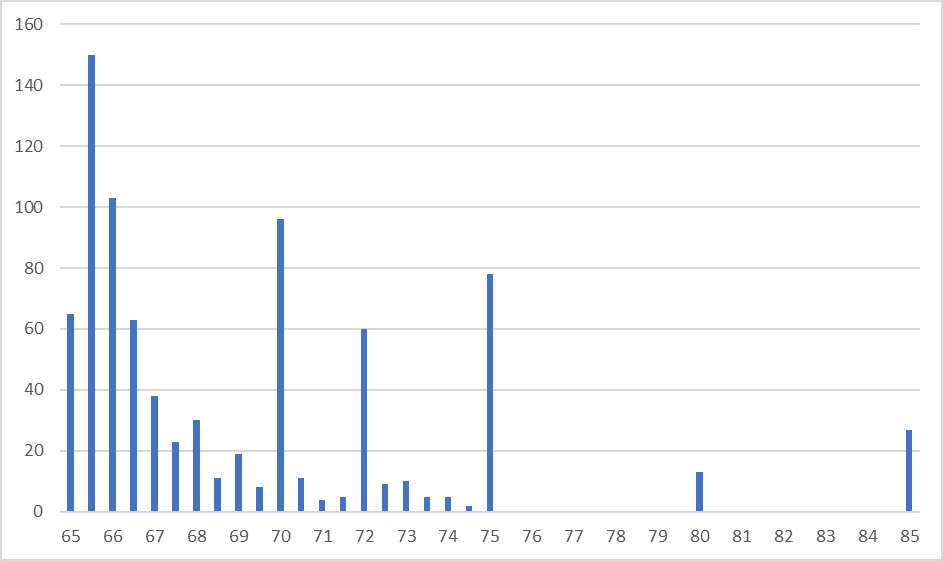
\includegraphics[width=.6\textwidth]{1.png}
	\caption{任务标价的统计}
\end{figure}

首先,我们需要确定是哪些因素影响到了定价。

我们首先对不同价格的点进行了可视化处理,下图中,绿色为低价65-70,黄色为中等价格,70-75,红色为高价75-85。我们可以发现,所有点都围绕着四个城市的市中心分布,由内向外价格逐渐升高。

\begin{figure}[!h]
	\centering
	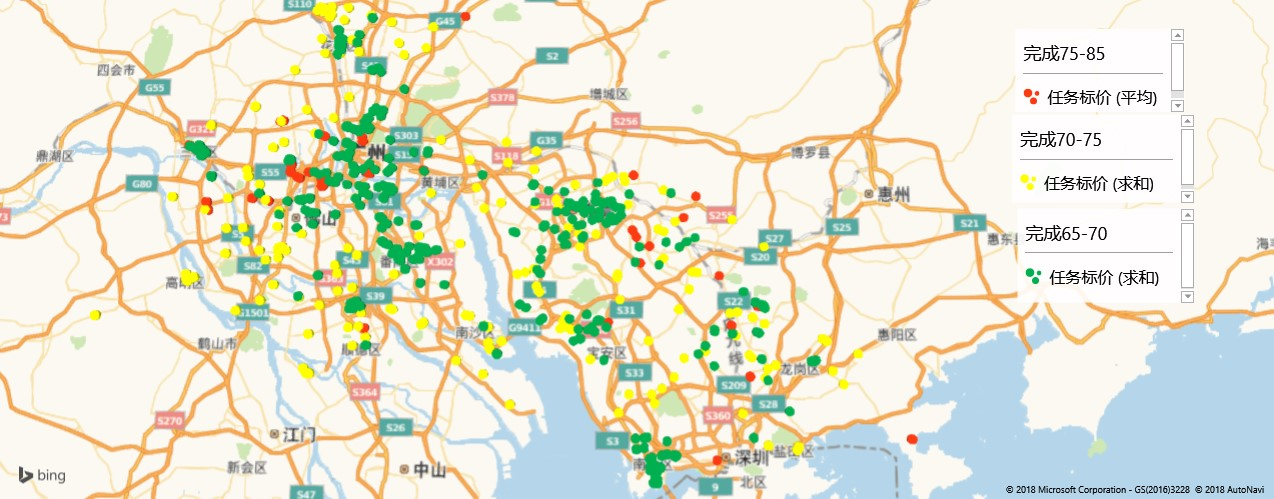
\includegraphics[width=.6\textwidth]{4.png}
	\caption{价格与地理位置的关系}
\end{figure}


我们认为,这一现象出现主要是因为由于会员的分布也是以市中心为中心逐渐向外扩散,当有更多会员的时候,APP更容易找到愿意接单的会员,所以会降低价格;而在郊区,由于会员较少,APP会选择提高价格,以增加会员接单的概率,因此我们猜想会员的密度为定价的主要因素之一。

\begin{figure}[!h]
	\centering
	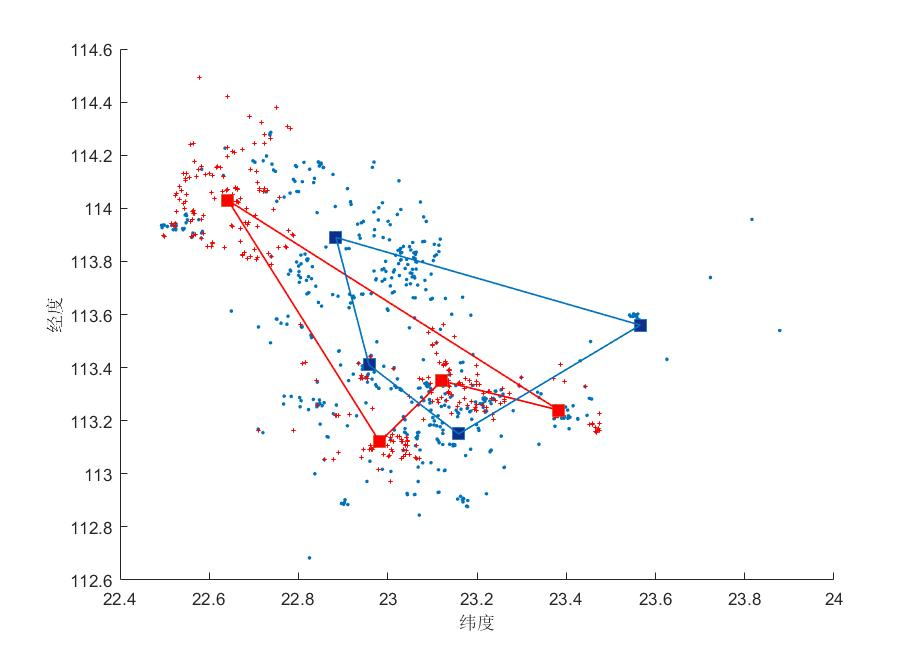
\includegraphics[width=.6\textwidth]{1.jpg}
	\caption{聚类分析}
\end{figure}


我们对数据点进行了聚类分析,发现无论是完成(蓝色)还是未完成(红色),四个聚类点都大致在四个市中心附近,说明四个市有明显的区域性特征。根据这一发现,我们对四个市的进行了统计。

\begin{table}[!htbp]
	\caption{各地概率值统计表}\label{tab001} \centering
	\begin{tabular}{lrrrr}
		\toprule[1.5pt]
		$ $    & {广州市} & {佛山市} & {深圳市} & {东莞市} \\
		\midrule[1pt]
		区域内任务数 & 318   & 175   & 164   & 177 \\
		任务完成数 & 193   & 116   & 35    & 177 \\
		任务未完成数 & 125   & 59    & 129   & 0 \\
		任务成功率 & 0.61  & 0.66  & 0.21  & 1 \\
		区域内会员数量 & 666   & 216   & 629   & 351 \\
		任务数/会员数 & 2.09  & 1.23  & 3.84  & 1.98 \\
		任务均价/元 & 68.07 & 71.42 & 67.33 & 70.34 \\
		人口(万) & 1350.11 & 743.06 & 1190.84 & 825.41 \\
		2016GDP & 19610.94 & 8630  & 19492.6 & 6827.67 \\
		面积    & 7434  & 3875  & 1996.85 & 2465 \\
		\bottomrule[1.5pt]
	\end{tabular}%
\end{table}
发现通过对四个城市的数据进行相关性分析,发现会员数量与任务标价相关系数为-0.97,说明会员数量与人物标价线性负相关,验证了我们之前的猜想。

\begin{table}[!htbp]
	\caption{各地概率值统计表}\label{tab001} \centering
	\begin{tabular}{lr}
		\toprule[1.5pt]
		& {与任务标价的相关系数} \\
		\midrule[1pt]
		该市内任务数 & -0.359 \\
		任务完成数 & 0.313558 \\
		任务未完成数 & -0.79595 \\
		任务成功率 & 0.700243 \\
		该市内会员数量 & -0.97389 \\
		\bottomrule[1.5pt]
	\end{tabular}%
\end{table}

同时,根据附件二的信息,我们发现信誉值与任务限额对定价也有一定的影响。一般信誉值越高,任务限额越高,说明该会员越老,对该APP的忠实度也就越高。而该APP为了吸引更多的新用户和培养忠实用户,一般它的定价算法会选择给新会员较高的定价,以提高会员的忠实度。


\subsubsection{问题一与问题二模型的解决}
对每一任务,根据经纬度至距离的转换公式
\begin{equation}
\left.
d=\frac{2\pi R}{360}\left[ \left(\phi_1-\phi_2\right)^2+  \left(\lambda_1-\lambda_2\right)^2cos^2\left(\left(\phi_1+\phi_2\right)^2\right)  \right]^{0.5}
\right.
\end{equation}
计算出距离各个会员的距离,从中选出100个最近的会员,取出这100个会员的距离,信誉值和任务限额的平均值作为这个任务的影响因素。然后对每一个成功完成的任务,计算出如上数据,利用多元线性回归得到回归方程。最后根据回归方程计算未完成的任务的期望定价,进行修正。


\begin{table}[!htbp]
	\caption{变量的含义}\label{tab001} \centering
	\begin{tabular}{lr}
		\toprule[1.5pt]
		& {与任务标价的相关系数} \\
		\midrule[1pt]
		$x_1$ & 最近的100个会员的平均距离 \\
		$x_2$ & 最近的100个会员的限额 \\
		$x_3$ & 最近的100个会员的信誉值 \\
		\bottomrule[1.5pt]
	\end{tabular}%
\end{table}

多变量线性预测模型如下
\begin{equation}
\left.
h_{\theta}(x) =\theta_0+\theta_1x_1+\theta_2x_2+\theta_3x_3+\theta_4x_4+... +\theta_n x_n
\right.
\end{equation}

转换为矩阵形式,则有两个向量,设$x_0=1$
\[x=\left[x_0\quad	x_1\quad	x_2\quad x_3	\quad	...\quad x_n \right]^T\]
\[\theta=\left[\theta_0\quad	\theta_1\quad	\theta_2\quad \theta_3	\quad	...\quad \theta_n \right]^T\]
预测函数为
\begin{equation}
\left.
h_\theta \left(x\right)=\theta^T·x
\right.
\end{equation}
代价函数为
\begin{equation}
\left.
J\left(\theta_0,\theta_1,\theta_2,\theta_n \right)=\frac{1}{2m}\sum_{i=1}^{n} \left(h_\theta\left(x_{\left(i\right)}\right)-y_{\left(i\right)}\right)^2
\right.
\end{equation}
用梯度下降计算方法,将
\begin{equation}
\left.
Repeat\theta_j:=\theta_j-\alpha\frac{1}{m} \sum_{i=1}^{m} \left(h_\theta\left(x_{\left(i\right)}\right)-y_{\left(i\right)}\right)
\right.
\end{equation}
最终我们得到对附近100人的平均距离、平均限额、平均信誉值多元线性拟合结果
\begin{equation}
\left.
h_\theta\left(x\right) = 67.1709 + x_1*0.4615 +x_2*(-0.0329)+x_3*(-0.001)
\right.
\end{equation}

\begin{figure}[!h]
	\centering
	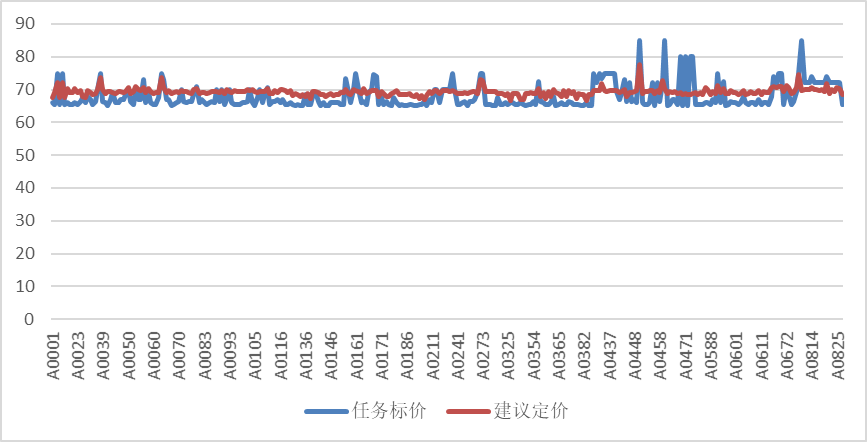
\includegraphics[width=.6\textwidth]{5.png}
	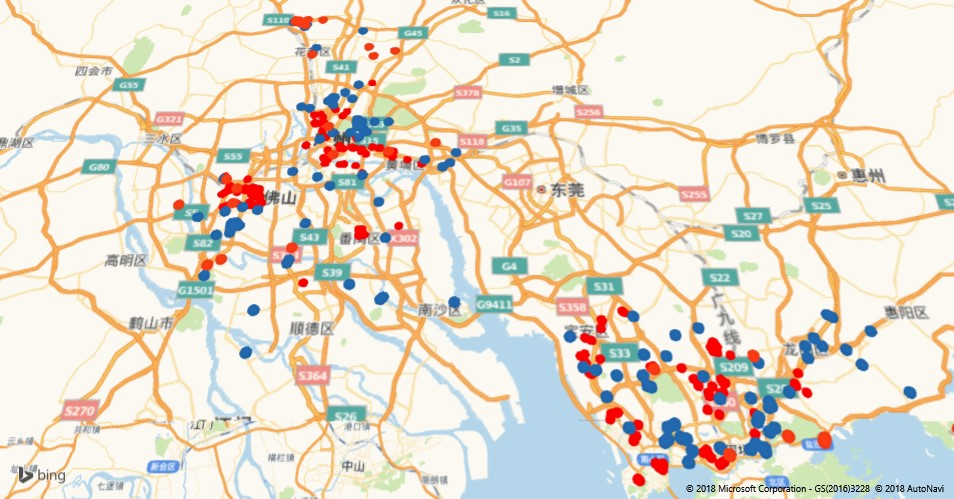
\includegraphics[width=.6\textwidth]{6.png}
	\caption{多元线性拟合结果(蓝色差值小于2.5)}
\end{figure}

\begin{table}[!htbp]
	\caption{拟合的部分结果}\label{tab001} \centering
	\begin{tabular}{lrr}
		\toprule[1.5pt]
		任务号码  & {任务标价} & {建议定价} \\
		\midrule[1pt]
		A0001 & 66    & 67.58338 \\
		A0002 & 65.5  & 69.09991 \\
		A0004 & 75    & 72.14669 \\
		A0005 & 65.5  & 67.48742 \\
		A0006 & 75    & 72.16929 \\
		A0008 & 65.5  & 67.45801 \\
		A0009 & 66    & 70.22592 \\
		A0011 & 65.5  & 68.9426 \\
		\bottomrule[1.5pt]
	\end{tabular}%
\end{table}
如图4和表4所示,我们的以平均距离、平均信誉值和平均限额为变量的多元线性拟合取得了比较满意的结果。但是我们同时发现我们的模型对郊区的高价任务标价有着较高的拟合度,而对市区的定价大多都高于原价。

从整体上对未完成订单的原因进行分析,在表1内对比,订单分布在四个市:广州、佛山、深圳、东莞。其中东莞的完成率最高,为100\%,深圳的完成率最低为21\%。而且每个市的任务总数与会员总数的比值在深圳最大,即相 比其他3个市,深圳的任务数最少,而会员数排第二,且接近排位第一的广州,分别是排位第三的东莞和 排位第四的佛山的2~3倍.拥有如此多会员,任务完成率却很低,可见这些会员虽然注册,但其信誉值 却较低.这说明只是偶尔接一两单任务,并不是该APP的忠实用户,整体上说明任务定价过低,不适用 于深圳.另一个原因可能是居住在深圳的人们生活节奏太快,空闲时间太少,虽然注册成为会员,但能有 时间做任务的人却远小于注册的会员数.做任务少导致信誉值低,因此任务的完成度应该与信誉值有关. 


\begin{table}[!htbp]
	\caption{各城市任务完成率与各因素的相关性}\label{tab001} \centering
	    \begin{tabular}{cc}
	    \toprule[1.5pt]
		 $ $&{相关系数} \\
		\midrule[1pt]
		会员数量  & -0.57949217 \\
		任务均价  & 0.700243079 \\
		人口    & -0.56224897 \\
		GDP(2016年) & -0.7873647 \\
		面积    & 0.083154688 \\
		\bottomrule[1.5pt]
	\end{tabular}%
\end{table}

我们发现完成率和任务均价的相关系数为正0.70,这说明,价格的确可以一定程度上激励会员完成任务。

我们还发现完成率与该城市GDP相关性为-0.78,这说明,分析比较表1所示4个城市的经济发展状况,深圳最发达,东莞最不发达.深圳 物价高,人们生活节奏快,工资水平高,因而人们选择去完成任务的概率较小.相反,东莞经济状况差,大 量工厂倒闭和裁员,流动人口减少,人们觉得做任务赚钱物有所值,因此东莞任务全部完成. 广州和佛山人们的生活水平较好,因此任务完成率处于中上等.另外,在广州和佛山市内部分析,发现两 个市的中心,即最繁华地带任务未完成几率远大于外围地区.可能是市中心人们生活节奏快,工资高,空 闲时间少,任务定价无法吸引人.外围地区恰好相反.


 
\subsection{问题三模型}
众包的主要参与者包括公司(任务请求人)和会员(任务完成人),他们通过任务 联系在一起。在本问题中,公司通过众包平台发布该项目所有任务的位置和标价,众包 平台根据会员的信誉度规定每个会员的预定任务开始时间和预定任务限额,会员自己想 要完成的任务,通过网络反馈给众包平台,众包平台再根据每位会员预定限额所占比例 进行任务配发,即当多个会员选择同一个任务时,将该任务分配给预定限额比例最大的 会员,会员接受任务后开始完成任务,将任务结果反馈给众包平台,公司通过平台审核 任务,将任务审核通过的会员信息反馈给众包平台,借助众包平台向该会员支付任务金 额。
\subsubsection{基于任务分布的打包模型}

对目前快递配送现状进行了分析,受到快递配送区域划分的启发,快递配送在划分 配送区域时,根据点密度选取初始聚类中心,基于这个思想本文对打包方案及算法做出 如下设计。
假设以$Q_i$ 为圆心的 500 米作为打包半径,该圆内包含的任务点个数记为$q_i$ , 如下可定义$Q_i$的点密度:
\[ \rho_i=q_i \]

设在未打包前的任务标号构成的集合为 $G_0$ ,计算该区域内任意一点$Q_i$ 的点密度 $\rho_i$ 
, 对点密度进行排序,找到使得$\rho_i$ 为最大点,记为$Q_0$ ,从$G_0$中删去 $Q_0$ 所对应的圆内 的$q_0$ 个任务点的标号,得到新的任务点标号集合,记为$G_1$ ;重新计算该区域内任意一点 的点密度并对其进行排序,找到最大点,记为 $Q_1$ ,从$G_1$ 中删去$Q_1$ 所对应圆 内的 $q_1$ 个任务点的标号,得到新的任务点标号集合,记为 $Q_2$ ,依次进行下去,直到该 区域内任意一点的点密度小于一阈值。

\subsubsection{打包定价分析}

在定价过程中,会员作为任务完成人构成一个群体,我们需要对该群体的行为进行 深入研究,达到对个体行为预测的目的,才能更好的与其他个体进行博弈。在本问题中 博弈双方为;公司和会员。在设计定价方案的过程中,需要从公司的角度去分析会员个体的行为,得出每个会 员个体对每个任务的综合作用效果,从此综合效果入手,确定最终的定价方案。

站在任务完成方的角度,第 i 个会员在预定任务时,对每个任务都以特定概率去预 定,记为 $P_i(C_j)$ 。当任务与会员的距离越近,标价越高时,会员预定该任务的概率越大,会员预定此任务的概率越大

通过上述分析知, $d_{ij}$越大表示任务点与会员的距离越远,会员完成该任务的概率越低,我们定义任务完成概率的距离影响因子为
\begin{equation}
\left.
\lambda_{12}=\frac{1}{e^{d_{ij}}}
\right.
\end{equation} 
同时,我们知道,定价越高,完成概率也越大,所以我们定义任务完成概率的定价影响因子为,价格分布的归一化处理后的结果
\begin{equation}
\left.
\sigma{j}=\frac{p-min(p)}{max(p)-min(p)}
\right.
\end{equation} 

站在定价方的角度,考虑在实际预定过程中,对某个特定的任务,每位会员都会以 一定的概率预定此任务,但我们关心的是此任务最终被预定的概率。假设$M_{ij}$ 表示第 j 个任务被第 i 个会员预定,那么该任务被预定的概率为 $P(M_{ij})$ 。
\begin{equation}
\left.
P(M_{ij})=\omega_1\lambda_{12}+\omega_2\sigma{j}
\right.
\end{equation}




在实际过程中,每位会员都可能会预定此任务,易得该任务被预定的概率等于会员 选择该任务的概率,即 $P_i(C_j)=P(M_{ij})$ 。

在实际会员完成任务的过程中,某个任务的预定概率较大并不能说明该任务会完成。因为每位会员的信誉值不同,导致会员完成该任务的概率小于该会员预定 此任务的概率。以下我们考虑受会员信誉值影响下的任务完成概率,设第 i 个会员完成 第 j 个任务的概率为: 

\begin{equation}
\left.
P\left( D_{ij}  \right)=P_i(C_j)+ f\left(\epsilon_i\right)
\right.
\end{equation}
其中其中 $\epsilon_i$ 表示第 i 个会员的信誉值
\begin{equation}
\left.f\left(\epsilon_i\right)=-\frac{1}{\epsilon_i}
\right.
\end{equation}
根据众包平台在分配任务时的分配原则,要使任务完成的总数越大,在分配任务时 应选择对应任务完成概率最大的会员,因此可知任务的完成概率:
\begin{equation}
\left.
P\left( D_{j}  \right)=max P\left( D_{ij} \right)
\right.
\end{equation}


\begin{equation}
\left.
P_j=\omega\left(\theta_0+\theta_1x_1+\theta_2x_2+\theta_3x_3\right)
\right.
\end{equation}

将任务打包后,任务包即视为一个任务点,将所有任务包与未打包任务点组合,并 重新编号,类比问题二中不含任务包的定价模型,建立如下含任务包的多目标规划模型
\[
min P_j
\]
\[
max p_j
\]
部分结果如下

\begin{table}[!htbp]
	\caption{ 部分任务包定价及被完成概率及定价}\label{tab001} \centering
\begin{tabular}{rrrr}
	\toprule[1.5pt]
	\multicolumn{1}{l}{任务包编号} & \multicolumn{1}{l}{ 任务包内任务个数 } & \multicolumn{1}{l}{任务包定价} & \multicolumn{1}{l}{ 任务包被完成概率 } \\
	\midrule[1pt]
	1     & 11    & 965.8604 & 0.541365 \\
	2     & 4     & 231.6592 & 0.864286 \\
	3     & 4     & 272.6422 & 0.586323 \\
	4     & 3     & 224.0409 & 0.927164 \\
		\bottomrule[1.5pt]
\end{tabular}%

\end{table}



\begin{table}[!htbp]
	\caption{ 全部被完成概率及总价}\label{tab001} \centering
    \begin{tabular}{lrr}
    \toprule[1.5pt]
	& \multicolumn{1}{l}{未打包的定价方案 } & \multicolumn{1}{l}{ 打包后的定价方案} \\
	\midrule[1pt]
	任务完成率  & 0.7122 & 0.8059 \\
	任务总标价  & 34112.74 & 36371.46 \\
		\bottomrule[1.5pt]
\end{tabular}%
\end{table}

通过上表可以看出,打包后的任务完成率有所提高,但是任务总标价比未打包时的 定价方案高,说明在此种定价方案设计中,可有效提高任务完成率,但对标价和的优化 效果不佳。

\subsection{问题四模型}

将附件三导入至PowerMap得到新任务点的分布图,发现任务点分布在广州 市、佛山市和深圳市。

\begin{figure}[!h]
	\centering
	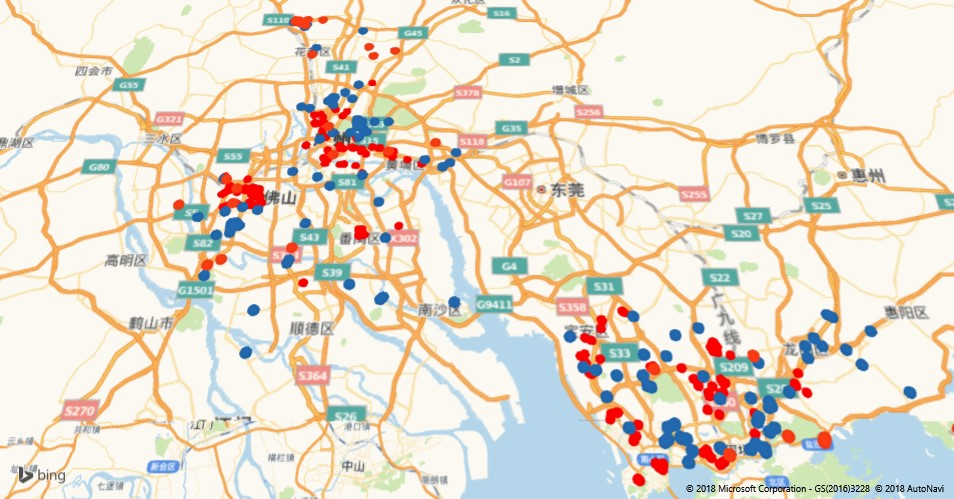
\includegraphics[width=.6\textwidth]{6.png}
	\caption{新任务的分布}
\end{figure}
将问题三的模型套入,我们发现,因为任务过于集中,很多任务包内含有20个以上的任务。任务包中任务个数很大,完成耗时长,会让任务包被完成概率低。因此我们设置了任务包内任务的上限为10个。
\begin{table}[!htbp]
	\caption{ 部分任务包的完成概率及总价}\label{tab001} \centering
	\begin{tabular}{rrrr}
		\toprule[1.5pt]
		\multicolumn{1}{l}{任务包编号} & \multicolumn{1}{l}{任务包内任务个数} & \multicolumn{1}{l}{任务包定价} & \multicolumn{1}{l}{任务包被完成概率} \\
		\midrule[1pt]
		1     & 13    & 948.9846 & 0.493162 \\
		2     & 10    & 611.4941 & 0.949166 \\
		3     & 10    & 487.4568 & 0.700086 \\
		4     & 9     & 530.8435 & 0.805416 \\
		\bottomrule[1.5pt]
	\end{tabular}%
\end{table}
总完成概率为0.507

\section{模型的改进}
本文在分析任务分配的过程中,未考虑每个会员开始预定时间的差异。实际上,由 于任务的分配原则,预定开始时间晚的会员在预定任务时会受到之前预定此任务会员的 影响,即在实际过程中,会员预定各任务的概率是随时间变化的。

在会员预定任务时,发现已经预定此任务的会员人数较大,就会导致该会员预定此 任务的概率变小,且该会员会更倾向于选择已经预定人数较少的任务。该现象表明,会 员预定某个任务的概率与其预定时刻任务点已有预定的会员数具有负相关性。 

因此,我们需要加入会员开始预定时间对众包任务的分配过程进行仿真模拟。

\section{模型的优缺点}
\subsection{模型的优点}
1、本文能有效量化标价及距离对任务完成情况的影响。 

2、在设计定价方案时,对个体行为进行了分析,使得出的标价与任务完成情况之 间的关系更加合理
\subsection{模型的缺点}

1、在分析定价规律时,仅从宏观角度考虑影响定价的因素,还需从任务点区域的 经济水平、交通状况等角度综合考虑对任务定价的影响。 

2、问题二中求解多目标规划模型的算法复杂度较高

3、本文对时间对任务的影响并没有很好的考虑,进一步用时间修正模型难度较大。


%参考文献


\bibliography{exam}
\bibliographystyle{is-unsrt}

%\begin{thebibliography}{99}%宽度9
% \bibitem{bib:one} 韩中庚,数学建模方法及其应用,北京:高等教育出版社,2009。 
% \bibitem{bib:two}姜启源,谢金星,叶俊,数学模型,北京:高等教育出版社,2003。 
% \bibitem{bib:three}龚纯,王正林,精通 MATLAB 最优化计算,北京:电子工业出版社,2012。 
% \bibitem{bib:four}卓金武,李必文,魏永生,秦健,MATLAB 在数学建模中的应用,北京:北京 航空航天大学出版社,2014。
%\end{thebibliography}

\newpage
%附录
\appendix
\section{主程序--matlab 源程序}
\begin{lstlisting}[language=matlab]
function [dist,xiane,xinyuzhi] = clac()
info_renwu = load('renwu_information.txt');
row = size(info_renwu,1);
col = size(info_renwu,2);
dist = zeros(row,1);
xiane  = zeros(row,1);
xinyuzhi = zeros(row,1);
dingjia = info_renwu(:,3);
for i = 1:row
[dist(i),xiane(i),xinyuzhi(i)]=variable(info_renwu,i); 
end

 \end{lstlisting}

\section{计算距离--matlab 源程序}
\begin{lstlisting}[language=matlab]
function dis = distance(wei1,jing1,wei2,jing2)
R = 6370;
%dis = asin(sqrt(sin((wei1-wei2)/2)^2+cos(wei1)*cos(wei2)*sin((jing1-jing2)/2)^2));
%dis = dis*2*R;
dis = 2*pi*R/360*((wei1-wei2)^2+(jing1-jing2)^2*cos((wei1+wei2)/2)^2)^0.5;

\section{聚类--matlab 源程序}
\begin{lstlisting}[language=matlab]
function [dist,xiane,xinyuzhi] = variable(info_renwu,i)
info_huiyuan = load('huiyuan_location.txt');
data_xiane = info_huiyuan(:,3);
data_xinyu = info_huiyuan(:,4);
data_wei = info_huiyuan(:,1);
data_jing = info_huiyuan(:,2);
num = size(data_jing,1);
data_distance = zeros(num,1);
sum = 0;
for j = 1:num
data_distance(j) = distance(info_renwu(i,1),info_renwu(i,2),info_huiyuan(j,1),info_huiyuan(j,2));
end
[a,b] = sort(data_distance);
first = b(1:30,:);
for count = 1:30
sum = sum + data_distance(first(count));
end
dist = sum/30;
sum = 0;
for count = 1:30
sum = sum + data_xiane(first(count));
end
xiane = sum/30;
sum = 0;
for count = 1:30
sum = sum + data_xinyu(first(count));
end
xinyuzhi = sum/30;

\end{lstlisting}






\end{document} 